\documentclass{ximera}
\title{Images and Graphs}


\begin{document}
\begin{abstract}
    A description of how images and graphs are rendered or included.
\end{abstract}
\maketitle
   
\section*{How Ximera renders Image and Graph Content}

There are several ways to embed graphics into Ximera document. One method is to use \verb|\includegraphics|. Here we see an included a JPEG and a PNG:

\begin{center}
  %https://commons.wikimedia.org/wiki/File:Lama_LLama_Alpaca_06.jpg
  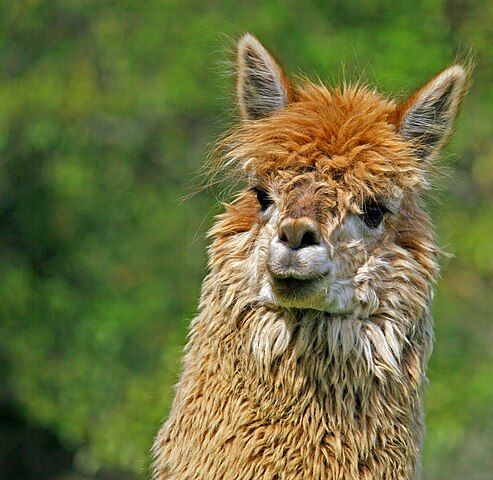
\includegraphics[width=.3\textwidth]{llama.jpg}\qquad
  %https://commons.wikimedia.org/wiki/File:Llama_in_watercolour.png
  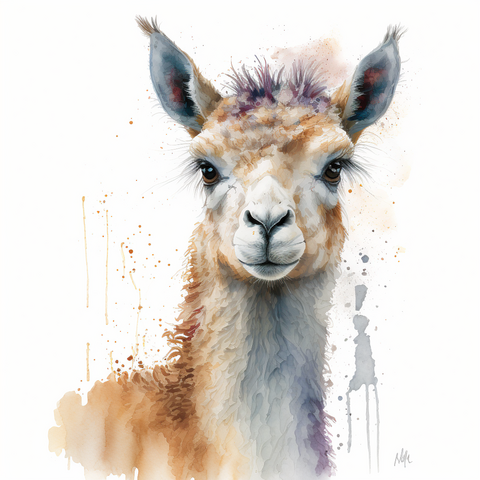
\includegraphics[width=.3\textwidth]{llama.png}
\end{center}

Here we have a pdf
\begin{center}
  
\includegraphics{llama.pdf}
\end{center}




    \subsection*{Any Necessary Content}
    
    
    
    \subsection*{Quirks of Rendering}
    
    
    
    \subsection*{Any Ximera-Specific Optional Arguments}
    
    
    
    \subsection*{Accessibility}
    
    
    
    \subsection*{Potential Problems and Pitfalls}
    
    
    
    \subsection*{Any Best Practices or Advice}
    
    

    
\end{document}
